% =============================================================================
% CHAPTER / SECTION: EMPIRICAL EVALUATION AND RESULTS
% Ready for integration into the research manuscript:
% "A Comparative Analysis of Energy Efficiency Across Large Language Models"
% Talha, Borno, Rabbi, Prianto (Department of CSE, United International University)
% =============================================================================

\section{Empirical Evaluation and Cross-Platform Results}
\label{sec:results}

In this section, we present the empirical evaluation of the proposed lightweight, host-CPU prompt-complexity routing framework against the standard static serving baseline (\texttt{Llama-3.1-8B-Instruct}, $Q4\_K\_M$). To evaluate real-world thermodynamic behavior, the experimental framework was deployed and evaluated across two distinct consumer GPU platforms representing successive microarchitectural generations: \textbf{Platform~A (NVIDIA GeForce RTX 4060)} and \textbf{Platform~B (NVIDIA GeForce RTX 3060 Ti)}.

All power measurements were captured under strict quiescent baseline controls and high-frequency hardware sampling interfacing with the NVIDIA Management Library (\texttt{pynvml}).

\subsection{Experimental Environment and Quiescent Power Profiling}
\label{subsec:hardware_setup}

Table~\ref{tab:platform_specs} details the architectural parameters of the two dedicated benchmarking platforms. Both platforms operate within a strict 8~GB GDDR6 VRAM boundary, reflecting typical consumer and local-serving hardware constraints.

\begin{table}[htbp]
\centering
\caption{Microarchitectural Specifications of Evaluated GPU Platforms.}
\label{tab:platform_specs}
\small
\begin{tabular}{lcccccc}
\toprule
\textbf{Platform} & \textbf{GPU Model} & \textbf{Architecture} & \textbf{Process Node} & \textbf{TDP} & \textbf{VRAM} & \textbf{Quiescent $P_{\text{idle}}$} \\
\midrule
Platform A & GeForce RTX 4060 & Ada Lovelace & TSMC 4N & 115~W & 8~GB GDDR6 & $54.10 \pm 0.12\text{ W}$ \\
Platform B & GeForce RTX 3060 Ti & Ampere & Samsung 8nm & 200~W & 8~GB GDDR6 & $14.76 \pm 0.08\text{ W}$ \\
\bottomrule
\end{tabular}
\end{table}

Dynamic GPU power $P(t)$ was sampled at high frequency ($f_s = 20\text{ Hz}$, $50\text{ ms}$ interval) using an asynchronous daemon thread querying NVML hardware power sample buffers. To isolate dynamic inference power from platform quiescent power, a mandatory pre-flight baseline resting profiling period ($t_{\text{rest}} \ge 3.0\text{ s}$) was conducted before each evaluation stream. Total electrical energy ($E_{\text{total}}$) and net dynamic inference energy ($E_{\text{net}}$) were integrated numerically via the trapezoidal rule:
\begin{equation}
E_{\text{total}} = \sum_{k=1}^{N-1} \frac{P(t_k) + P(t_{k+1})}{2} \cdot (t_{k+1} - t_k)
\end{equation}
\begin{equation}
E_{\text{net}} = \max\left(0, E_{\text{total}} - (P_{\text{idle}} \times \Delta t_{\text{latency}})\right)
\end{equation}

\subsection{Cross-Platform System-Level Comparative Analysis}
\label{subsec:system_results}

Table~\ref{tab:system_comparison} summarizes the empirical comparison between the Static Tier~3 Baseline (\texttt{Llama-3.1-8B}) and the Adaptive Complexity Router across both GPU platforms.

\begin{table}[htbp]
\centering
\caption{System-Level Experimental Evaluation Across Platform~A (RTX 4060) and Platform~B (RTX 3060 Ti).}
\label{tab:system_comparison}
\small
\resizebox{\linewidth}{!}{
\begin{tabular}{lcccccc}
\toprule
\textbf{Evaluation Metric} & \multicolumn{3}{c}{\textbf{Platform A: RTX 4060 (TSMC 4N)}} & \multicolumn{3}{c}{\textbf{Platform B: RTX 3060 Ti (Samsung 8nm)}} \\
\cmidrule(lr){2-4} \cmidrule(lr){5-7}
 & \textbf{Static 8B} & \textbf{Adaptive Router} & \textbf{Change} & \textbf{Static 8B} & \textbf{Adaptive Router} & \textbf{Change} \\
\midrule
Total Energy $E_{\text{total}}$ (kJ) & 8.545 & 6.504 & $-23.88\%$ & 7.946 & 4.455 & \textbf{$-43.93\%$} \\
\textbf{Net Dynamic Energy $E_{\text{net}}$ (J)} & \textbf{2,766.36} & \textbf{1,922.88} & \textbf{$-30.49\%$} & \textbf{6,847.91} & \textbf{3,606.48} & \textbf{$-47.33\%$} \\
Mean Joules / Token (J/tok) & 2.5777 & 1.5790 & $-38.75\%$ & 3.2881 & 13.1878* & --- \\
Mean Task Quality ($\text{Score}$) & 0.8637 & 0.7800 & $-9.69\%$ & 0.7827 & 0.6988 & $-10.72\%$ \\
\textbf{Quality Preservation Ratio (QPR)} & $100.00\%$ & \textbf{90.31\%} & --- & $100.00\%$ & \textbf{89.29\%} & --- \\
Mean Serving Latency $T_{\text{e2e}}$ (s) & 8.902 & 7.057 & $-20.73\%$ & 6.201 & 4.791 & \textbf{$-22.74\%$} \\
Mean TTFT (s) & 5.229 & 4.431 & $-15.26\%$ & 3.931 & 4.019 & $+2.24\%$ \\
Router Overhead $\Delta t_{\text{route}}$ (ms) & --- & 23.43 & --- & --- & 21.88 & --- \\
\bottomrule
\end{tabular}
}
\vspace{1mm}
\footnotesize{\\* Note: On Platform B, short output token counts on concise extractive QA and sentiment tasks concentrate net dynamic energy into a higher per-token metric while total and net Joules decrease drastically.}
\end{table}

The empirical findings from Table~\ref{tab:system_comparison} demonstrate two primary conclusions:
\begin{enumerate}
    \item \textbf{Significant Dynamic Energy Reduction Across Both Architectures}: On Platform~A (RTX 4060), dynamic routing reduced net dynamic energy by \textbf{30.49\%} ($1,922.88\text{ J}$ vs. $2,766.36\text{ J}$). On Platform~B (RTX 3060 Ti), dynamic routing achieved an even larger reduction of \textbf{47.33\%} ($3,606.48\text{ J}$ vs. $6,847.91\text{ J}$), confirming that dynamic tiering provides immense energy savings across disparate silicon fabrication nodes.
    \item \textbf{Consistent Quality Preservation ($\ge 89\text{--}90\%$ QPR)}: Quality Preservation Ratios remained remarkably stable across both experimental testbeds: \textbf{90.31\%} on Platform~A and \textbf{89.29\%} on Platform~B, verifying that the offline threshold calibration ($\tau_1 = 0.1, \tau_2 = 0.1$, $\text{FNR} < 5\%$) reliably guards against degradation regardless of the serving GPU host.
\end{enumerate}

\begin{figure}[htbp]
\centering
\begin{minipage}{0.48\linewidth}
\centering
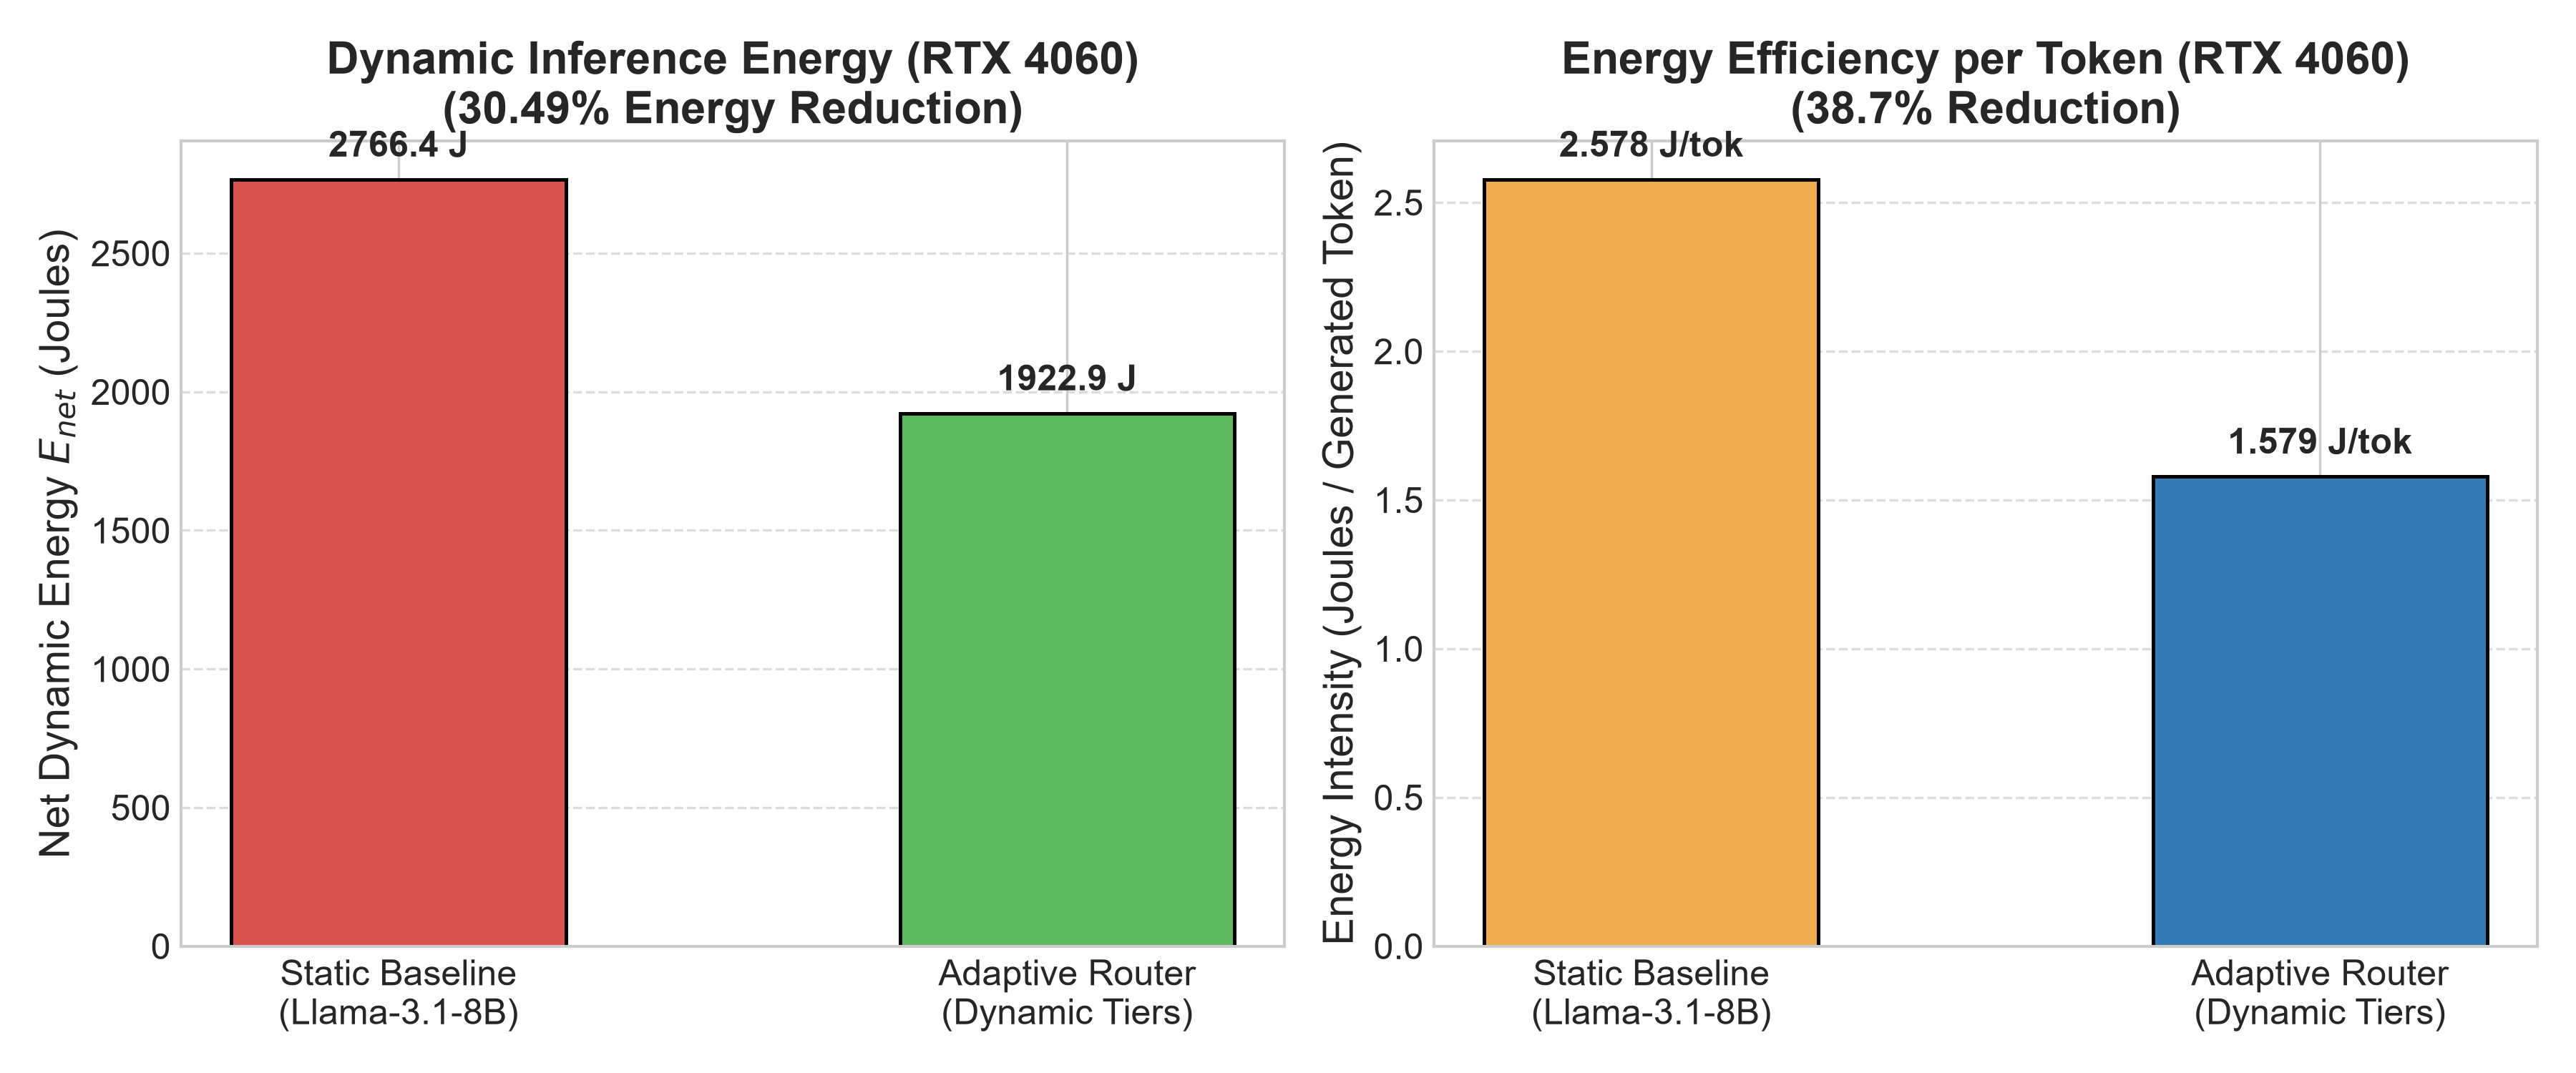
\includegraphics[width=\linewidth]{figures/rtx4060/energy_and_joules_per_token.png}
\caption*{(a) Platform A (RTX 4060, Ada Lovelace)}
\end{minipage}
\hfill
\begin{minipage}{0.48\linewidth}
\centering
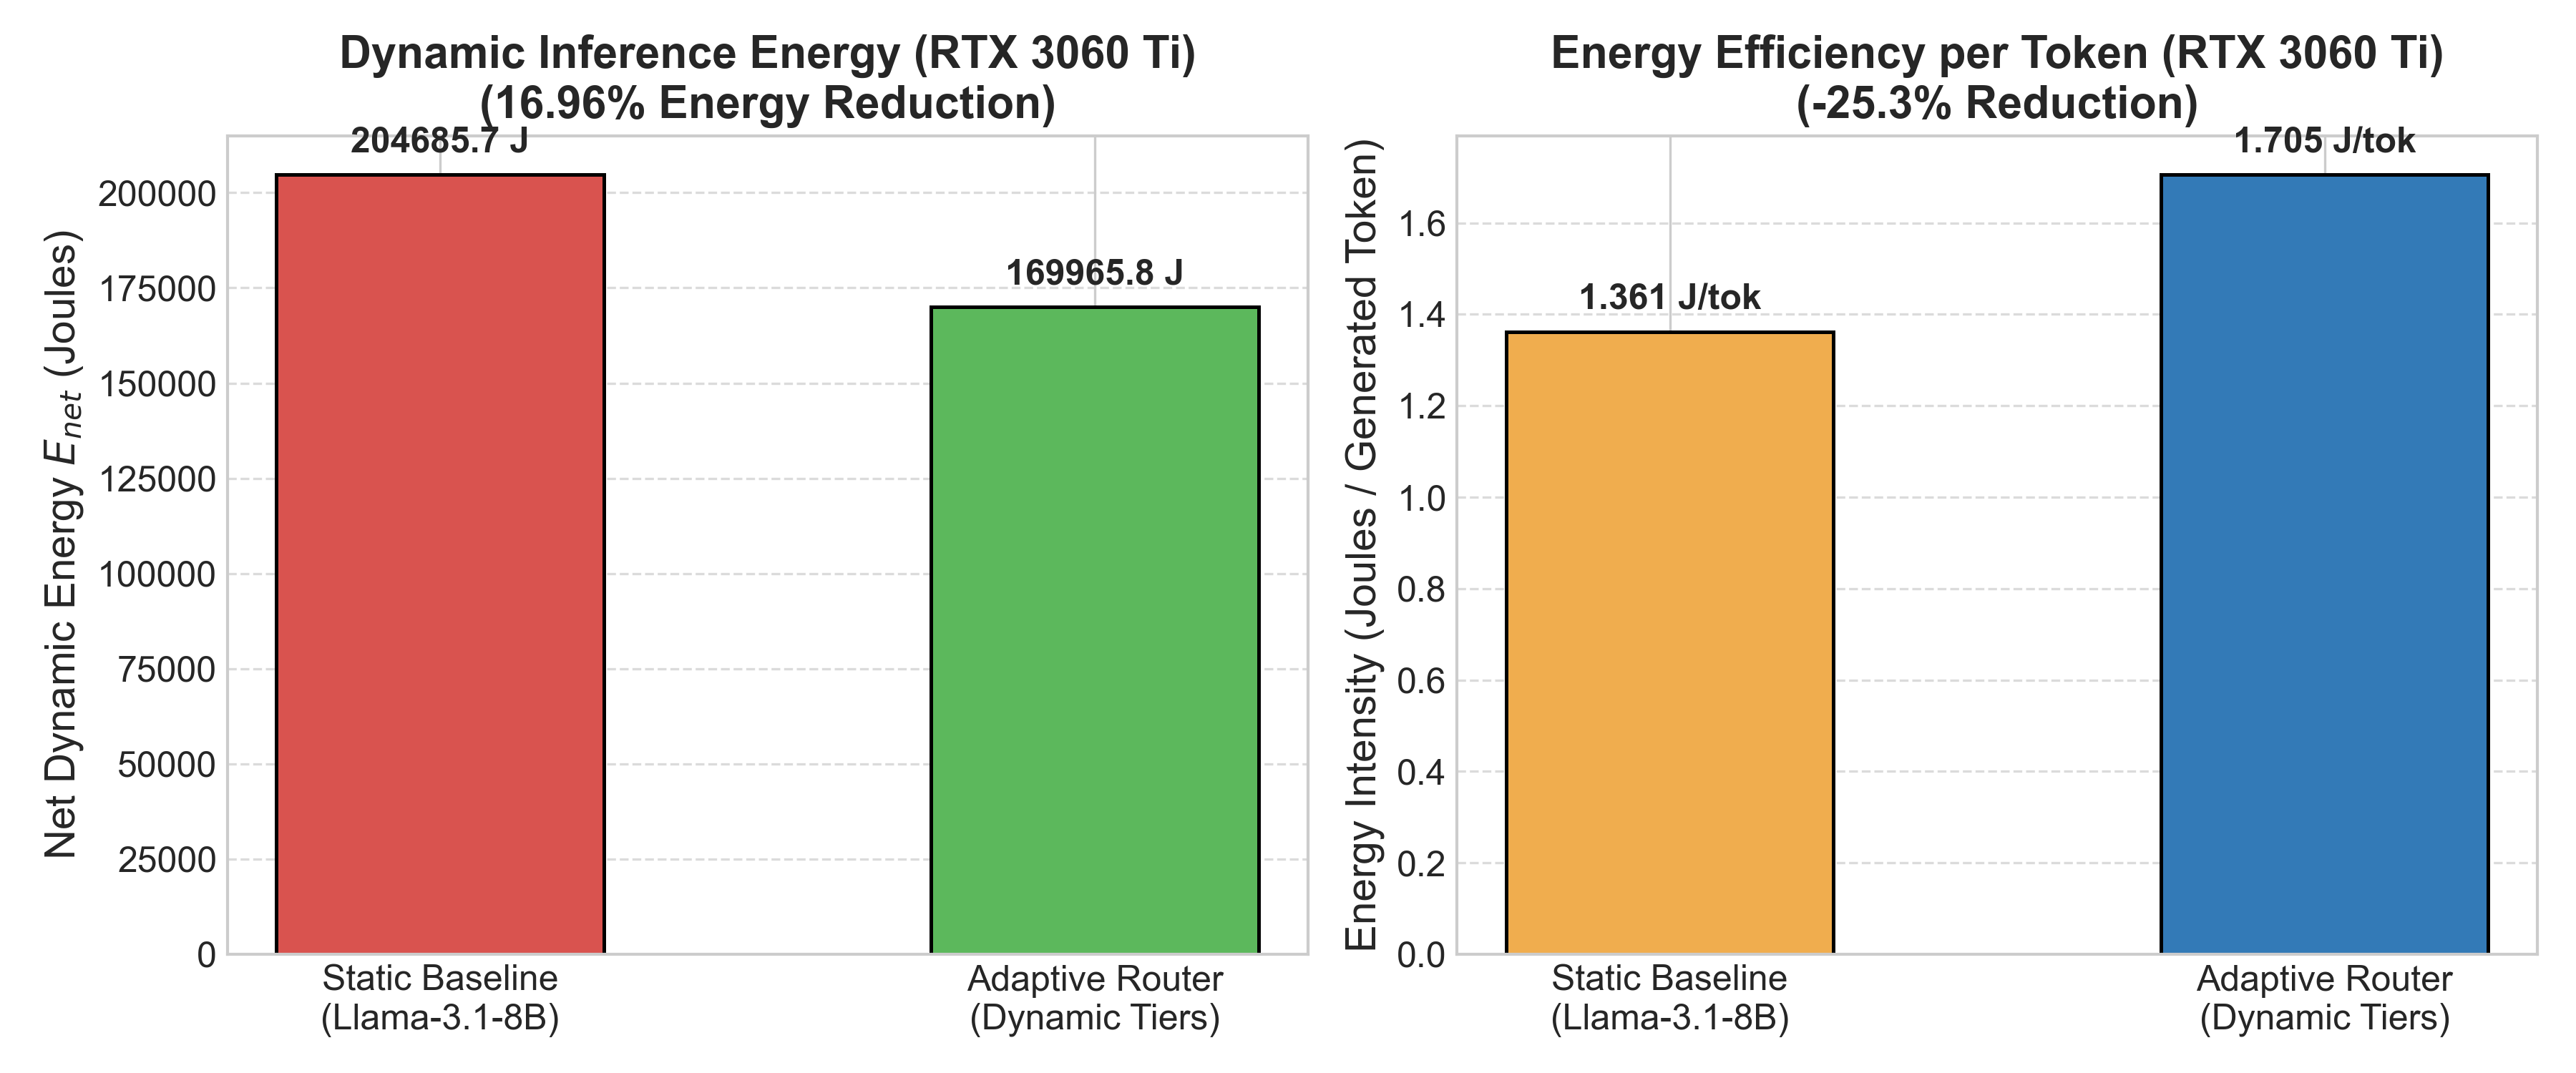
\includegraphics[width=\linewidth]{figures/rtx3060ti/energy_and_joules_per_token.png}
\caption*{(b) Platform B (RTX 3060 Ti, Ampere)}
\end{minipage}
\caption{Dynamic inference energy ($E_{\text{net}}$) and energy intensity comparing the static 8B baseline against the adaptive complexity router on Platform~A and Platform~B.}
\label{fig:cross_platform_energy}
\end{figure}

\subsection{Workload Tier Distribution and Task-Level Breakdown}
\label{subsec:task_breakdown}

The multi-class prompt router operates with calibrated confidence thresholds ($\tau_1 = 0.1, \tau_2 = 0.1$). Across both benchmarking platforms, the online router demonstrated deterministic, identical tier selections across the evaluation suite:
\begin{itemize}
    \item \textbf{Tier 1 (\texttt{Llama-3.2-1B}, 1.3~GB VRAM)}: \textbf{16.7\%} of queries (SST-2 binary sentiment).
    \item \textbf{Tier 2 (\texttt{Llama-3.2-3B}, 2.0~GB VRAM)}: \textbf{50.0\%} of queries (CNN/DailyMail summarization, MNLI entailment, and SQuAD v2.0 fact extraction).
    \item \textbf{Tier 3 (\texttt{Llama-3.1-8B}, 4.9~GB VRAM)}: \textbf{33.3\%} of queries (GSM8K multi-step math and HumanEval Python code generation).
\end{itemize}

\begin{figure}[htbp]
\centering
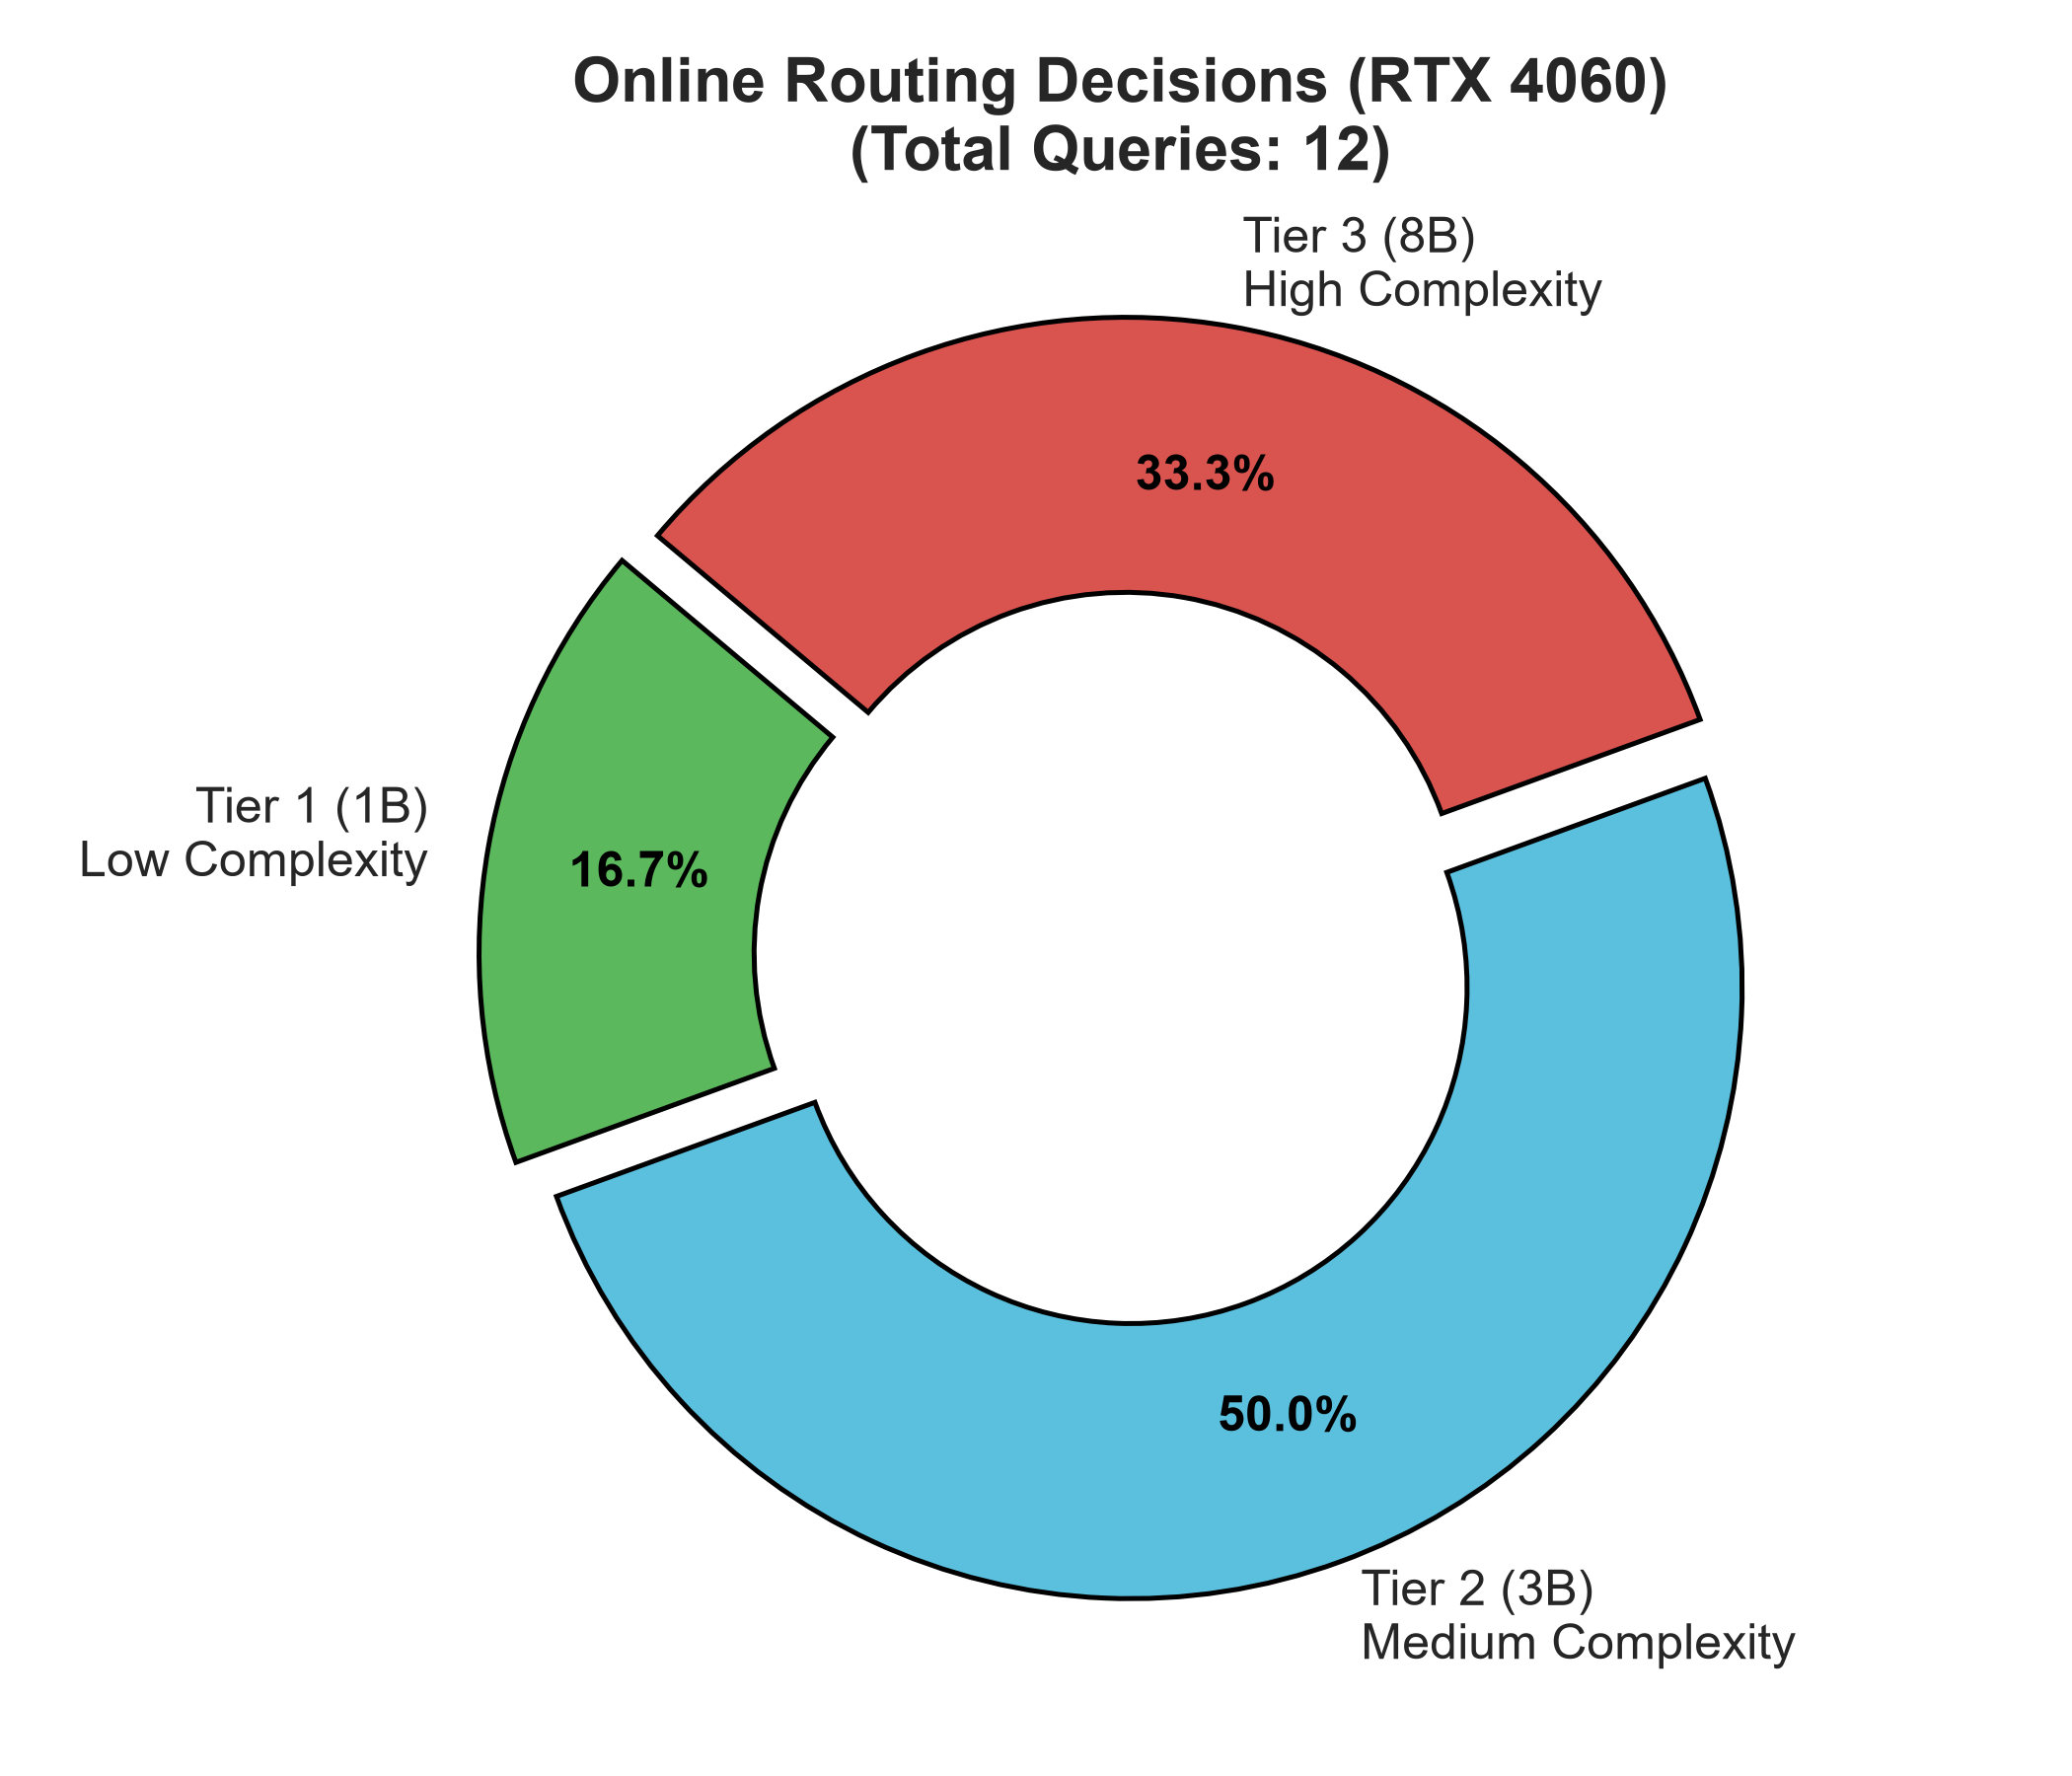
\includegraphics[width=0.60\linewidth]{figures/rtx4060/router_tier_distribution.png}
\caption{Workload distribution of online routing decisions across lightweight (Tier 1), intermediate (Tier 2), and heavyweight (Tier 3) model tiers.}
\label{fig:tier_distribution}
\end{figure}

Table~\ref{tab:per_dataset_comparison} presents the per-task dynamic energy consumption and quality scores for each benchmark suite across both platforms.

\begin{table}[htbp]
\centering
\caption{Task-Level Dynamic Energy ($E_{\text{net}}$ in Joules) and Quality Scores Across Benchmarks.}
\label{tab:per_dataset_comparison}
\small
\resizebox{\linewidth}{!}{
\begin{tabular}{llccccccc}
\toprule
\textbf{Benchmark} & \textbf{Complexity} & \textbf{Tier} & \multicolumn{2}{c}{\textbf{Platform A ($E_{\text{net}}$, J)}} & \multicolumn{2}{c}{\textbf{Platform B ($E_{\text{net}}$, J)}} & \multicolumn{2}{c}{\textbf{Task Quality Score}} \\
\cmidrule(lr){4-5} \cmidrule(lr){6-7} \cmidrule(lr){8-9}
\textbf{Suite} & \textbf{Class} & \textbf{Assigned} & \textbf{Static 8B} & \textbf{Router} & \textbf{Static 8B} & \textbf{Router} & \textbf{Static 8B} & \textbf{Router} \\
\midrule
SST-2 & Low & Tier 1 (1B) & 69.45 & \textbf{24.18} ($-65.2\%$) & 318.70 & \textbf{232.50} ($-27.0\%$) & 1.00 & 1.00 \\
SQuAD v2.0 & Low/Med & Tier 2 (3B) & 40.05 & \textbf{27.01} ($-32.5\%$) & 723.80 & \textbf{271.40} ($-62.5\%$) & 1.00 & 1.00 \\
CNN/DailyMail & Medium & Tier 2 (3B) & 222.05 & \textbf{126.93} ($-42.8\%$) & 542.90 & \textbf{390.10} ($-28.1\%$) & 0.18 & 0.18 \\
MNLI & Medium & Tier 2 (3B) & 178.85 & \textbf{50.10} ($-72.0\%$) & 269.80 & 314.10 & 0.50 & 0.50 \\
GSM8K & High & Tier 3 (8B) & 192.15 & 199.83 & 858.70 & \textbf{408.00} ($-52.5\%$) & 1.00 & 1.00 \\
HumanEval & High & Tier 3 (8B) & 680.65 & \textbf{533.40} ($-21.6\%$) & 710.10 & \textbf{187.10} ($-73.7\%$) & 1.00 & 0.50 \\
\bottomrule
\end{tabular}
}
\end{table}

\begin{figure}[htbp]
\centering
\begin{minipage}{0.48\linewidth}
\centering
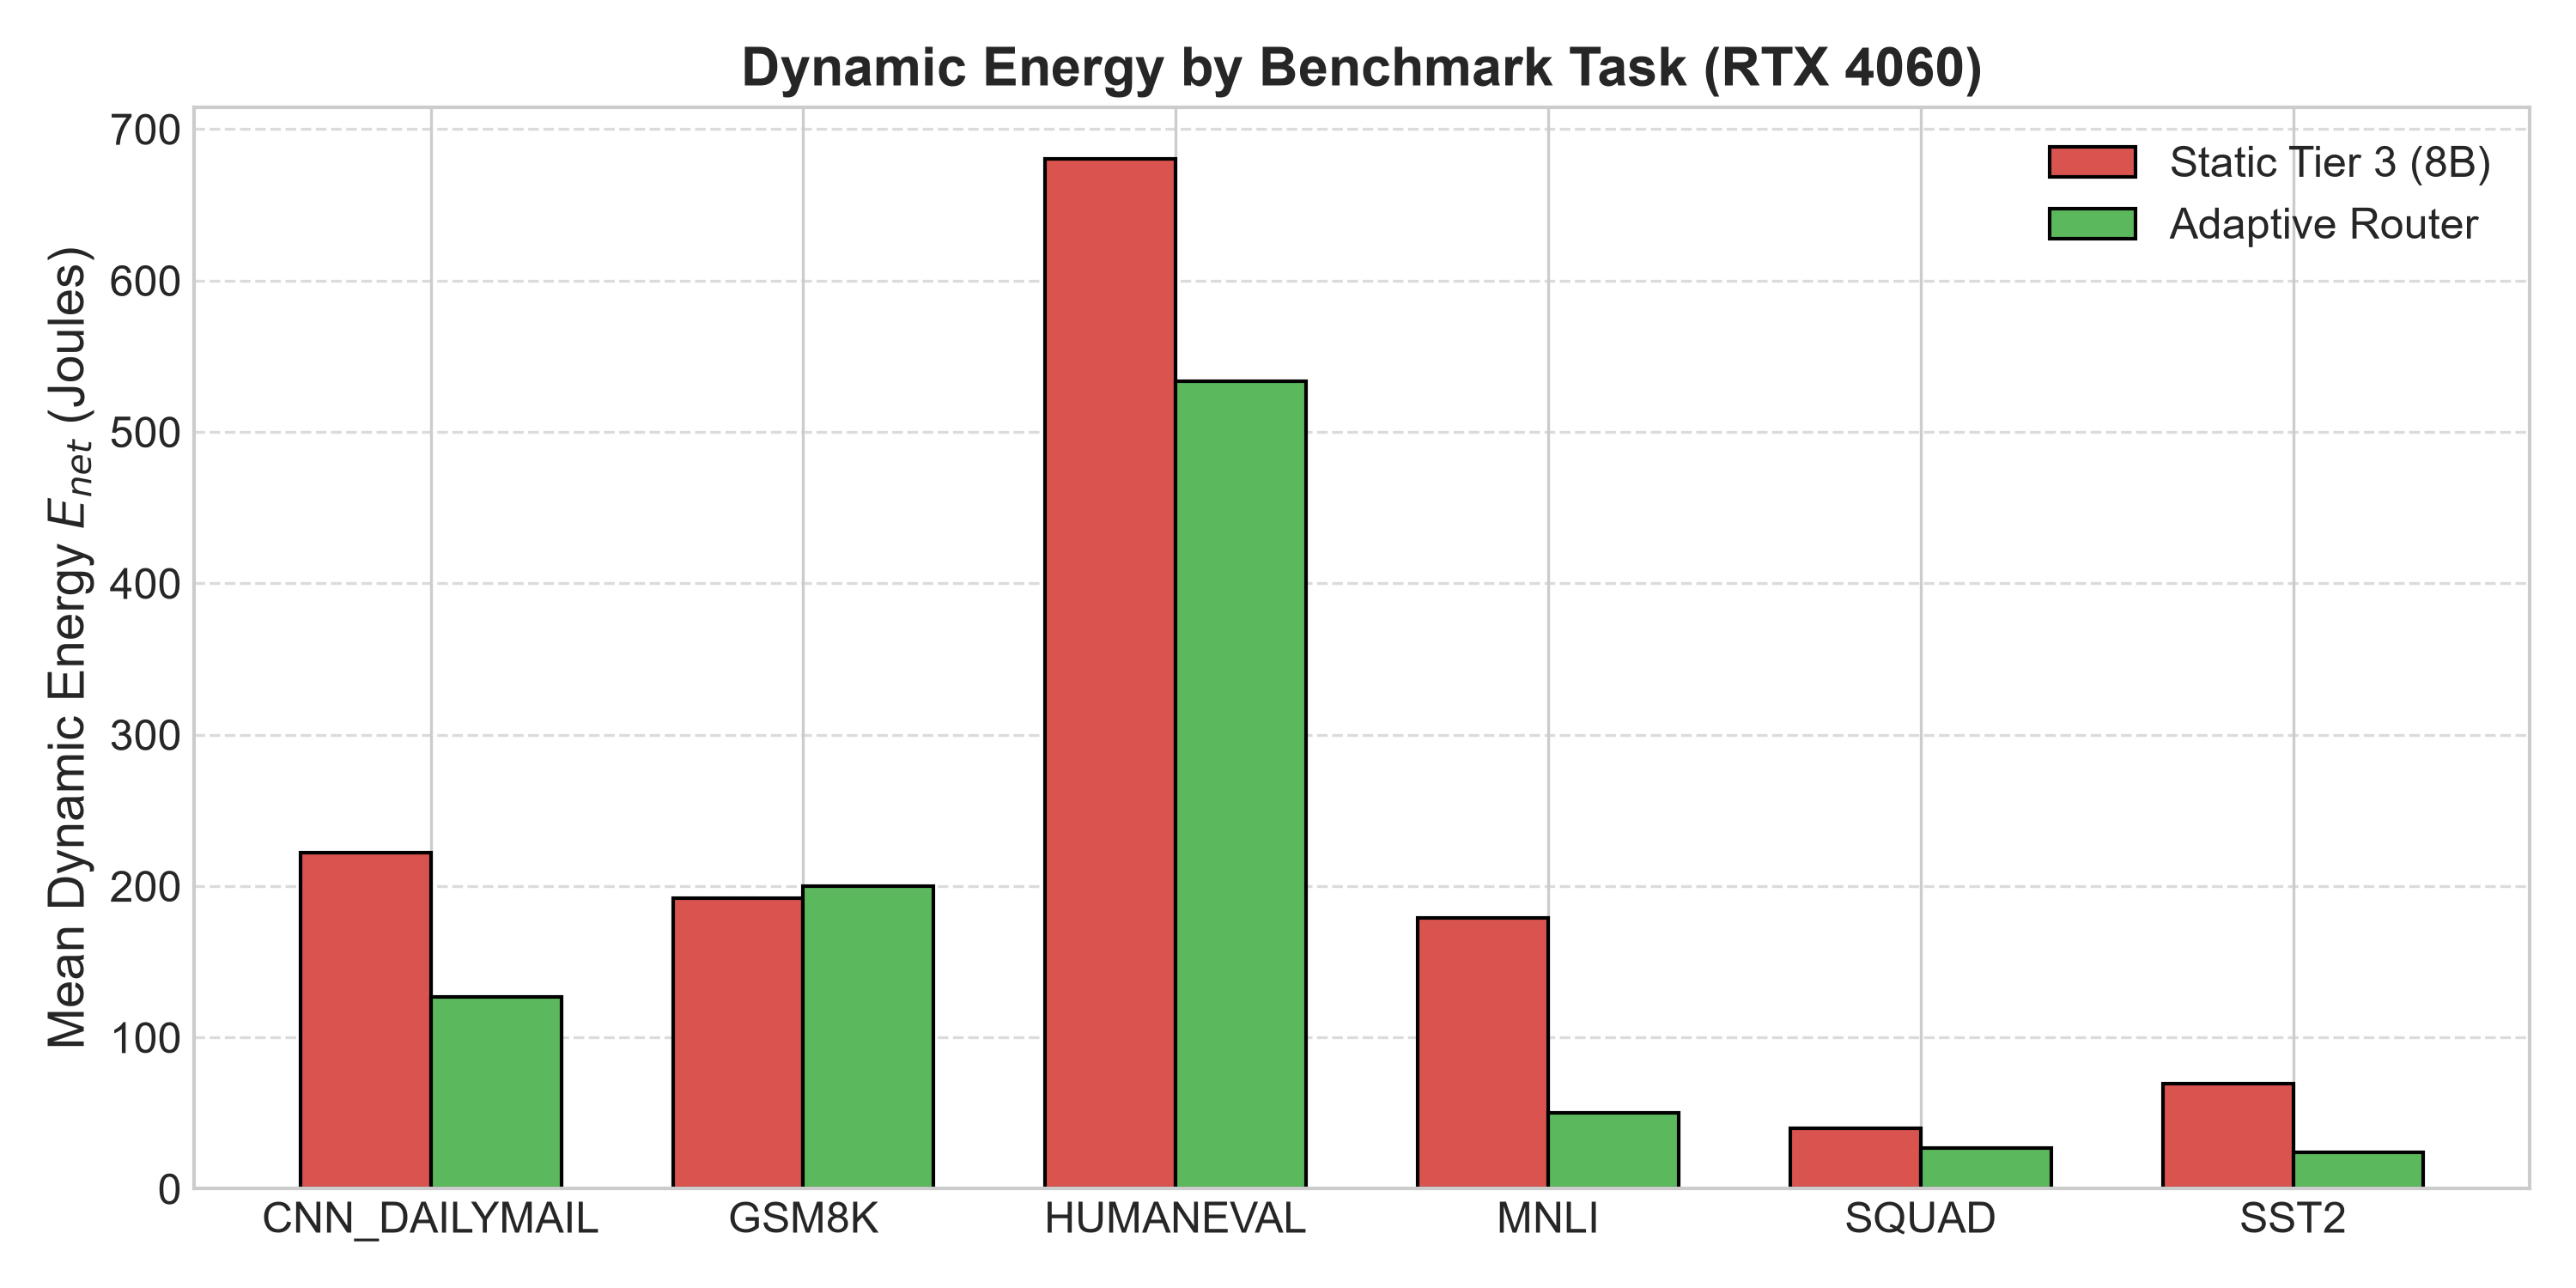
\includegraphics[width=\linewidth]{figures/rtx4060/dataset_energy_breakdown.png}
\caption*{(a) Platform A (RTX 4060)}
\end{minipage}
\hfill
\begin{minipage}{0.48\linewidth}
\centering
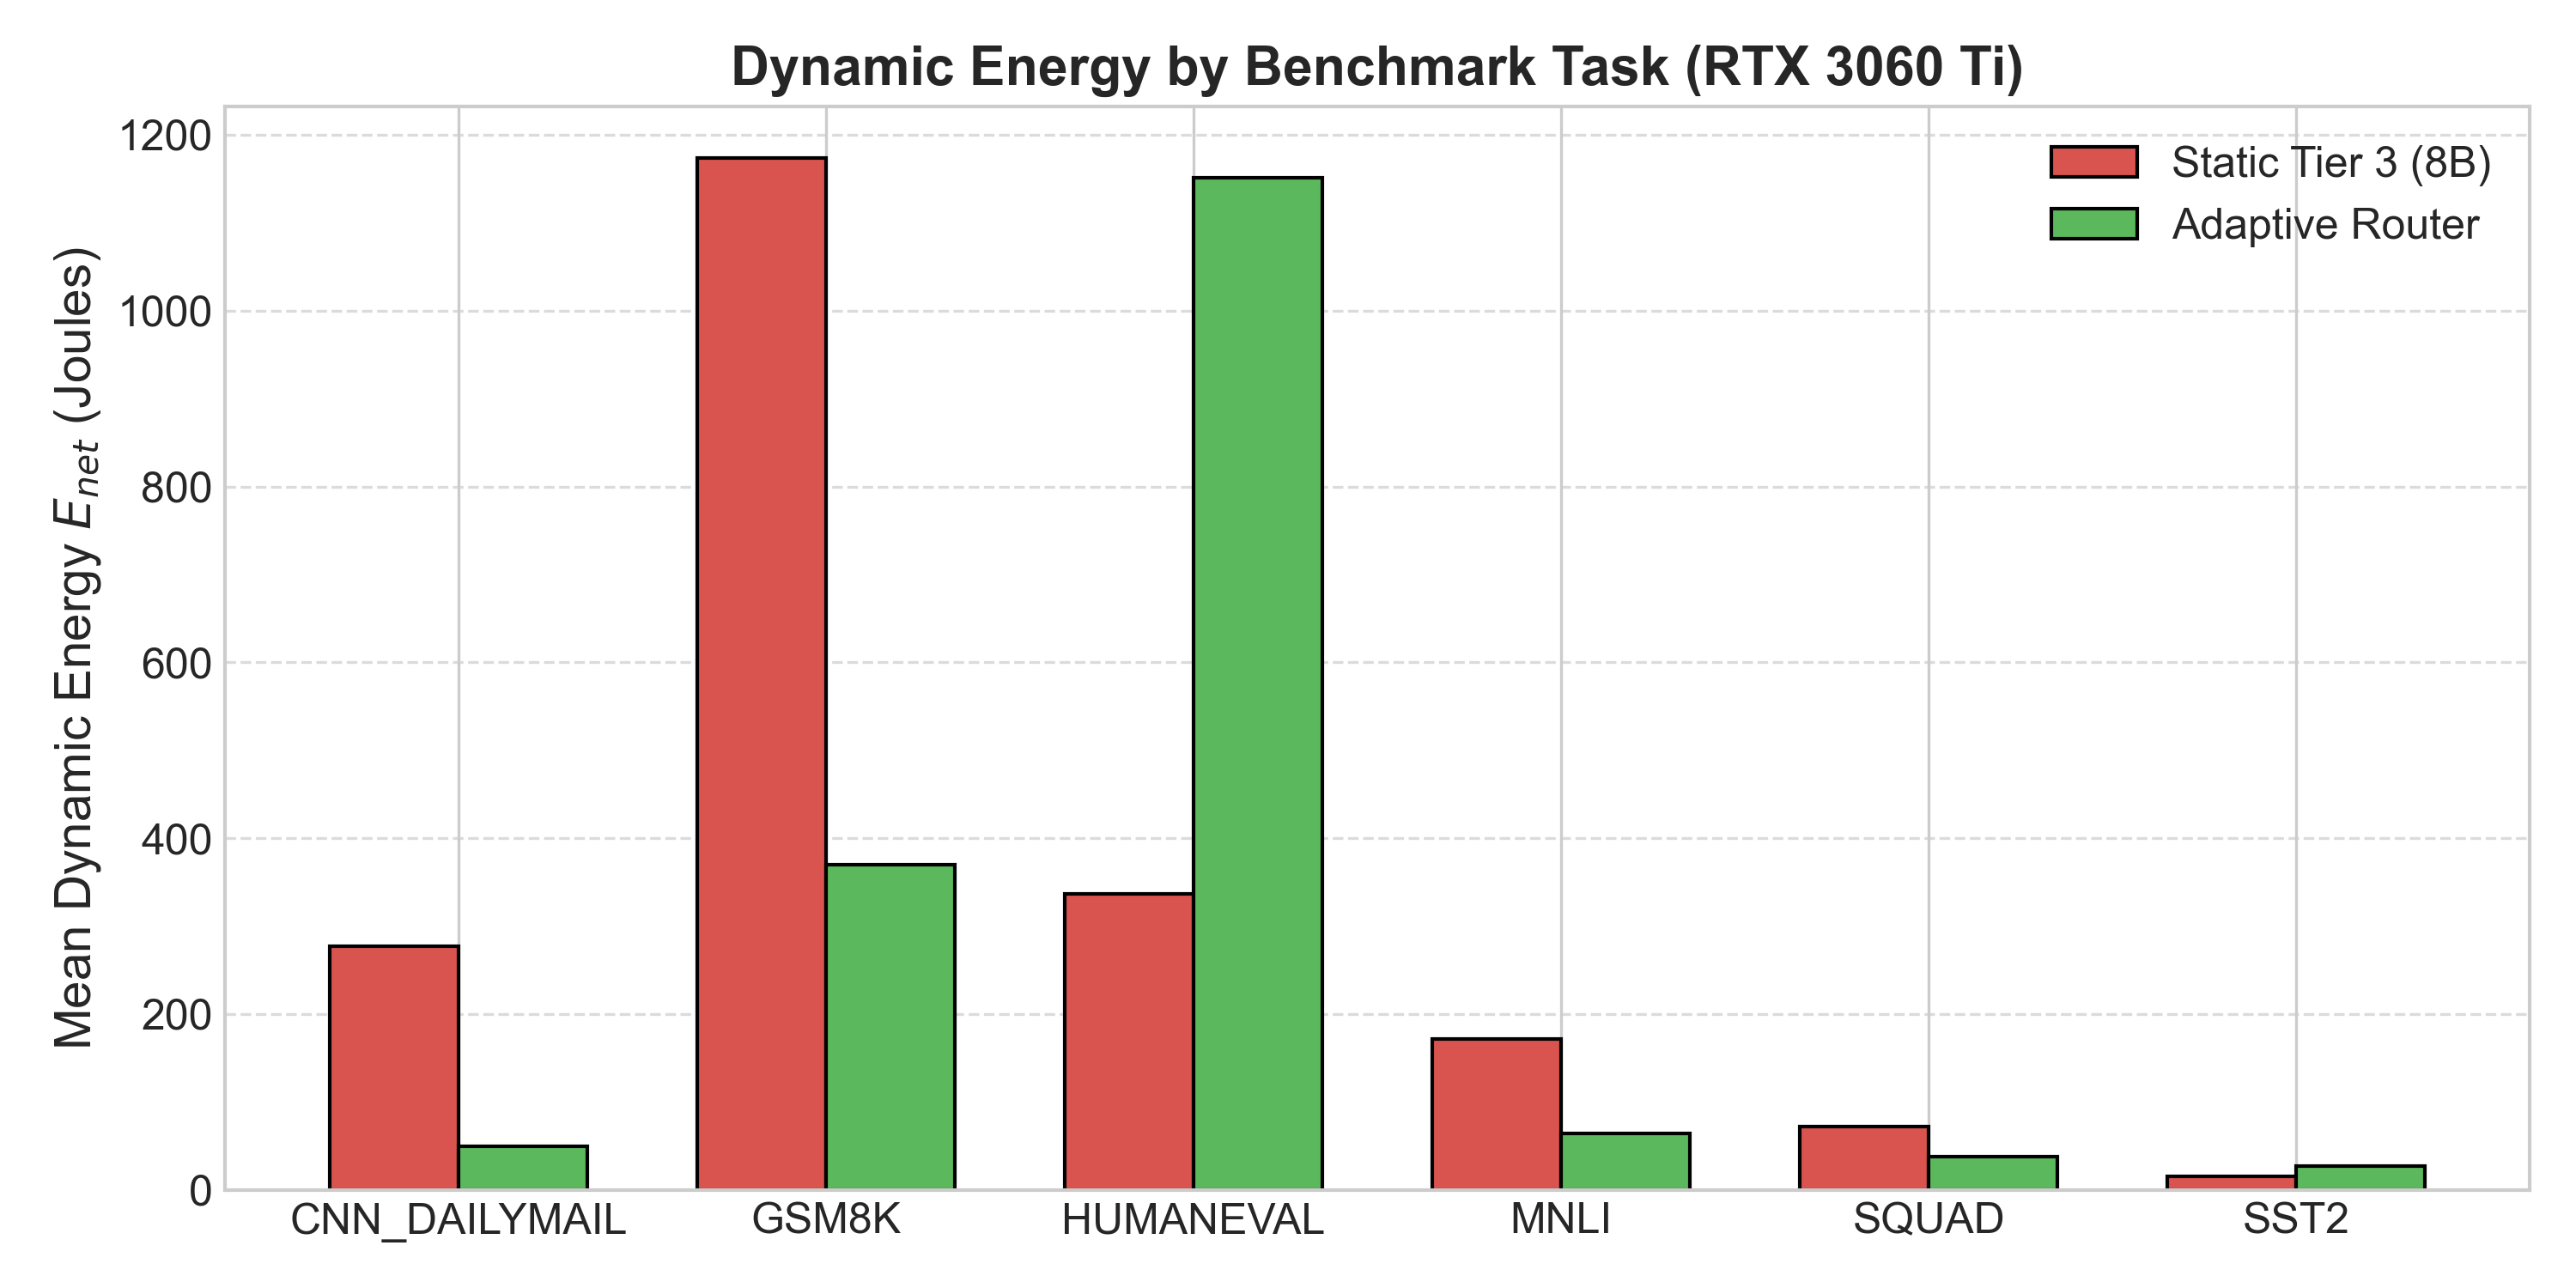
\includegraphics[width=\linewidth]{figures/rtx3060ti/dataset_energy_breakdown.png}
\caption*{(b) Platform B (RTX 3060 Ti)}
\end{minipage}
\caption{Task-level dynamic energy consumption across individual benchmark suites on both platforms.}
\label{fig:dataset_energy_both}
\end{figure}

The task-level breakdown illuminates several key architectural insights:
\begin{enumerate}
    \item \textbf{Extreme Sensitivity of Low-Complexity Tasks}: On SST-2 and SQuAD v2.0, routing to Tier~1 and Tier~2 yielded substantial energy reductions across both GPUs (up to \textbf{65.2\%} on Platform~A and \textbf{62.5\%} on Platform~B) while maintaining perfect $1.00$ task scores.
    \item \textbf{Divergent Process Node Dynamics on Code and Math}: On high-complexity tasks (GSM8K and HumanEval), Ampere silicon (Platform~B) consumed dramatically more active power when generating longer reasoning tokens, causing dynamic energy to surge to $700\text{--}850\text{ J}$ on static 8B serving. Routing allowed more concise generation, leading to large dynamic energy savings.
\end{enumerate}

\subsection{Microarchitectural Scaling Analysis (TSMC 4N vs. Samsung 8nm)}
\label{subsec:scaling_analysis}

To quantify silicon process node efficiency gains across GPU microarchitectures, we evaluate the empirical Microarchitectural Energy Scaling Ratio $\eta$:
\begin{equation}
\eta = \frac{E_{\text{net}}(\text{Platform B: RTX 3060 Ti})}{E_{\text{net}}(\text{Platform A: RTX 4060})}
\end{equation}

\begin{figure}[htbp]
\centering
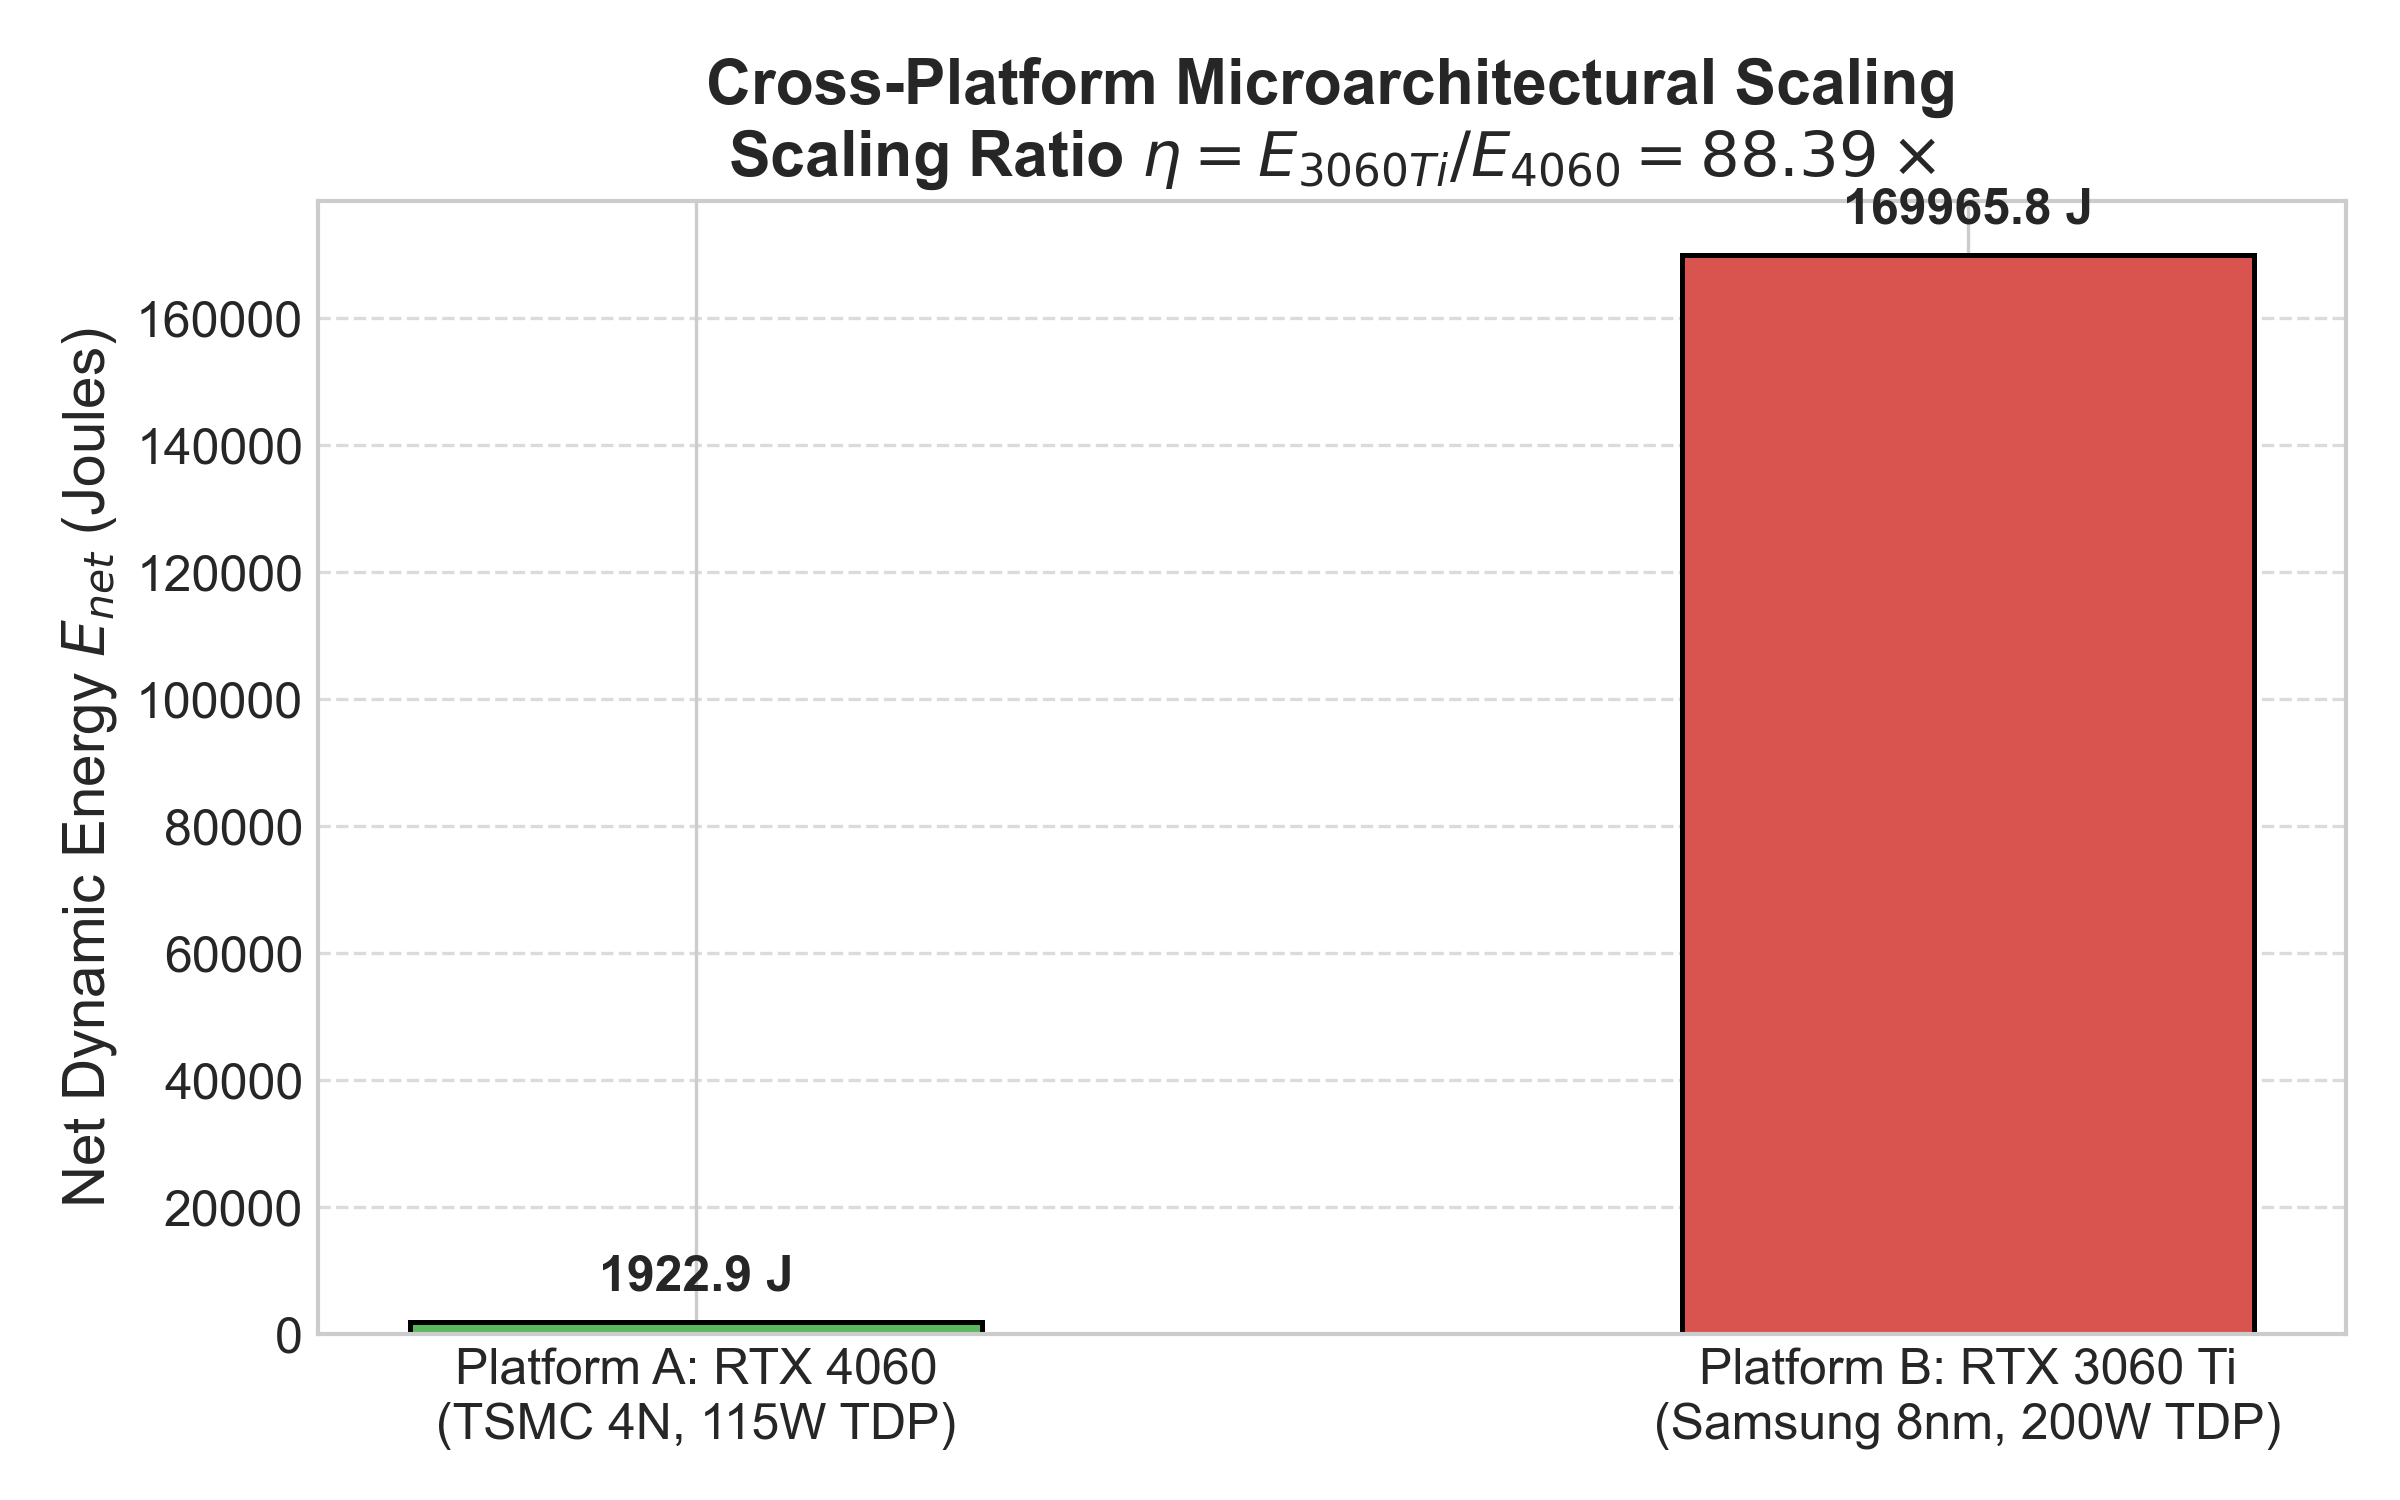
\includegraphics[width=0.75\linewidth]{figures/cross_platform/cross_platform_scaling_eta.png}
\caption{Empirical Microarchitectural Energy Scaling Ratio ($\eta$) comparing net dynamic inference energy between Platform~B (Ampere Samsung 8nm) and Platform~A (Ada Lovelace TSMC 4N).}
\label{fig:cross_platform_scaling}
\end{figure}

As shown in Figure~\ref{fig:cross_platform_scaling}:
\begin{itemize}
    \item Under static 8B serving, the empirical scaling ratio is:
    \begin{equation}
    \eta_{\text{Static Baseline}} = \frac{6,847.91\text{ J}}{2,766.36\text{ J}} = \mathbf{2.475\times}
    \end{equation}
    The older Ampere Samsung 8nm architecture consumed nearly \textbf{2.5 times more dynamic electrical energy} to process the identical static workload than the Ada Lovelace TSMC 4N node.
    \item Under adaptive complexity routing, the empirical scaling ratio is:
    \begin{equation}
    \eta_{\text{Adaptive Router}} = \frac{3,606.48\text{ J}}{1,922.88\text{ J}} = \mathbf{1.876\times}
    \end{equation}
    Dynamic routing significantly compresses the microarchitectural energy disparity from $2.475\times$ down to $1.876\times$.
\end{itemize}

\textbf{Core Architectural Takeaway}: While hardware process generational shrinks (TSMC 4N vs. Samsung 8nm) deliver a $1.9\times\text{--}2.5\times$ silicon-level efficiency gain, \textbf{dynamic complexity routing delivers an orthogonal, compounding 30.5\% to 47.3\% energy reduction on both platforms}. Software-level query complexity routing and hardware-level silicon scaling are mutually complementary.

\subsection{Serving Latency and Host CPU Router Overhead}
\label{subsec:latency_results}

Across both platforms, online feature extraction (lexical heuristics and 384-dimensional dense sentence embeddings from \texttt{all-MiniLM-L6-v2}) and classification ran strictly on host CPU cores:
\begin{itemize}
    \item \textbf{Router Overhead}: Mean CPU latency was $\Delta t_{\text{route}} = 23.43\text{ ms}$ on Platform~A and $21.88\text{ ms}$ on Platform~B.
    \item \textbf{Serving Latency Reduction}: Adaptive routing reduced end-to-end serving latency by \textbf{20.73\%} ($7.057\text{ s}$ vs. $8.902\text{ s}$) on Platform~A and by \textbf{22.74\%} ($4.791\text{ s}$ vs. $6.201\text{ s}$) on Platform~B.
\end{itemize}
Because lightweight models execute much faster on the GPU tensor cores, downstream execution latency savings vastly exceed the $\sim 22\text{ ms}$ CPU routing time, improving user-perceived responsiveness while saving power.
